\documentclass[10pt,a4paper]{article}
\usepackage[T1]{fontenc}
\usepackage{lmodern,microtype}
\usepackage{amsmath,amssymb,booktabs,graphicx,array,geometry,enumitem,hyperref,xcolor}
\geometry{left=1.65cm,right=1.65cm,top=1.5cm,bottom=1.55cm}
\setlength{\parindent}{0pt}
\setlength{\parskip}{3.5pt}
\setlist{nosep,leftmargin=*}
\hypersetup{colorlinks=true,urlcolor=blue!55!black,linkcolor=black}
\newcommand{\ESN}{\mbox{ESN A2-981003}}
\title{\vspace{-1.2em}\textbf{Path-Dependent Volatility with Echo State Networks}\\[-.15em]
\large Repository summary and numerical-validation status}
\author{Project summary generated from the repository sources and protocol reports}
\date{29 August 2026}
\begin{document}
\maketitle
\vspace{-1.4em}

\begin{abstract}\small
This repository is the numerical-validation component of a research programme on whether reservoir computing can provide a tractable model of path-dependent stochastic volatility.  Its central object is \ESN, a two-layer echo-state-network volatility model.  Five standalone Python protocols generate paths from known stochastic-volatility data-generating processes (DGPs), calibrate the ESN and benchmark models with a common multi-statistic objective, and save figures and LaTeX reports.  The work provides encouraging, but not conclusive, evidence that the ESN can reproduce several market stylised facts.  In particular, the numerical architecture selection and some fitted read-out effects remain noisy and require higher-budget multi-seed confirmation.
\end{abstract}

\section{What is in the repository}
There is no application package or automated test suite.  The five independent scripts each contain simulation, statistics, calibration, plotting, and report-writing code; their tracked PNG, JSON, \texttt{.tex}, and PDF outputs document historical runs.

\begin{center}\small
\begin{tabular}{p{4.75cm}p{3.55cm}p{6.35cm}}
\toprule
Folder & DGP / reference & Question tested \\
\midrule
\shortstack[l]{\texttt{GridSearch\_}\\\texttt{HyperParameters\_}\\\texttt{Tuning}} & fBM log-normal SV (rough and persistent), MRW, rough Bergomi & Shared ESN hyperparameters and reservoir dimensions \\
\texttt{Roughness} & fBM log-normal SV & Hurst roughness, covariance scaling, monofractality \\
\texttt{Taylor\_Effect} & Multifractal Random Walk (MRW) & Whether $\mathrm{ACF}(|r|)>\mathrm{ACF}(r^2)$ \\
\texttt{Leverage\_Effect} & Strong-leverage Heston & Negative $\mathrm{Corr}(r_t,V_{t+L})$ \\
\texttt{Zumbach\_Effect} & 4-factor Guyon--Lekeufack PDV & Time-reversal asymmetry of volatility/magnitude \\
\bottomrule
\end{tabular}
\end{center}

All comparisons use Gaussian innovations.  Except in the Zumbach protocol, which uses PDV--GL as its DGP and therefore compares ESN with QRH only, the candidate models are the ESN, quadratic rough Heston (QRH), and the two-factor path-dependent-volatility model of Guyon--Lekeufack (PDV--GL).

\section{Model under study: a finite-dimensional path-dependent reservoir}
The ESN combines a fast/slow linear reservoir $r\in\mathbb R^{N_r}$ with a nonlinear feedback bank $z\in\mathbb R^{N_z}$.  The $r$ modes have geometrically spaced mean-reversion rates and share one innovation $\varepsilon_t\sim\mathcal N(0,1)$:
\begin{equation}
 \lambda_i=\lambda_{\rm lo}\left(\frac{\lambda_{\rm hi}}{\lambda_{\rm lo}}\right)^{\frac{i-1}{N_r-1}},\qquad
 r_{i,t}=e^{-\lambda_i\Delta t}r_{i,t-1}+\sqrt{1-e^{-2\lambda_i\Delta t}}\,\varepsilon_t. \tag{1}
\end{equation}
Their common shock makes $q^\top r_t$ a sum-of-exponentials, Markovian approximation to a Volterra/fractional memory kernel.  The normalized read-out direction is based on the calibrated internal memory exponent $H_{\rm ESN}$:
\begin{equation}
 \tilde q_i=\lambda_i^{1/2-H_{\rm ESN}},\qquad
 q=\frac{\tilde q/\|\tilde q\|_2}{\sqrt{(\tilde q/\|\tilde q\|_2)^\top C(\tilde q/\|\tilde q\|_2)}},\quad q^\top Cq=1. \tag{2}
\end{equation}
Here $H_{\rm ESN}$ is \emph{not} the DGP Hurst parameter; it is an ESN calibration variable selected to match the realised roughness statistic.

The slower $z$ bank is a nonlinear filter of fast$\times$slow $r$ taps, with a \texttt{tanh} activation, even (variance-like), linear (leverage-like), self, and neighbouring-mode terms.  This construction is intended to give the model a controlled source of nonlinear multiscale and Zumbach-like effects.  The volatility read-out is
\begin{equation}
 \eta_t=b_0+\rho_r\,a_r(q^\top r_t)+\sum_{j=1}^{N_z}w_{j,z}z_{j,t}+r_t^\top Qr_t,\qquad
 \sigma_t=\sqrt{\sigma_{\min}^2+\operatorname{softplus}(\eta_t)^2}, \tag{3}
\end{equation}
\begin{equation}
 w_{j,z}=\frac{\operatorname{geomspace}(z_{\rm lo},z_{\rm hi},N_z)_j}{\sqrt{N_z}},\qquad
 Q=\frac{1}{N_r}(m_1I+m_2qq^\top),\qquad
 dX_t=(\mu-\tfrac12\sigma_t^2)+\sigma_t\varepsilon_t. \tag{4}
\end{equation}
The same innovation drives return and reservoir.  Fixing $\rho_r=-1$ and $a_r>0$ enforces a negative instantaneous leverage direction $\kappa_0=\rho_ra_rq^\top\sqrt{2\lambda}<0$.  This is a structural ESN mechanism rather than a fitted return/variance correlation.

The current reported architecture has $N_r=96$, $N_z=12$ and seven shared nonlinear-reservoir hyperparameters: $z$ strength 0.1929, even strength 2.2291, linear strength 0.1930, gate damping 0.9651, local $z$ coupling 0.0476, self-coupling scale 0.0397, and negative-sign probability 0.2219.  Per DGP, a 12-dimensional vector---memory/rate ranges, bias and scale, rough amplitude, two $z$ read-out endpoints, and $(m_1,m_2)$---is fitted by 11-start Nelder--Mead.

\section{Calibration and diagnostic methodology}
Each path is reduced to an 11-component stylised-fact vector: estimated Hurst exponent; mean, tail, and maximum volatility; volatility persistence; Taylor gap and fraction; Zumbach statistic; leverage; excess kurtosis; and maximum return autocorrelation.  DGP cross-path means and dispersions define the target.  Candidate models minimise the smooth score
\begin{equation}
 S=\sum_{k=1}^{11}w_k\left[1-f(x_k;c_k,s_k)\right]+5\,\mathrm{Stress},\qquad
 f(x;c,s)=\exp\!\left[-\tfrac12\left(\frac{x-c}{s}\right)^2\right]. \tag{5}
\end{equation}
Thus $S\geq0$ and $S=0$ is a perfect non-stressed match.  The Gaussian proximity replaced an earlier tent kernel because its gradient remains non-zero when a candidate is far from target.  The protocol being studied deliberately raises the associated weight/tightens tolerance: Taylor components in the Taylor experiment, leverage in the Heston experiment, and the two Zumbach channels in the PDV experiment.

The DGPs are meaningful controlled tests.  For example, roughness uses
\begin{equation}
 \sigma_t=\sigma_0\exp\!\left(\lambda B_t^H-\tfrac12\lambda^2t^{2H}\right),\qquad
 \operatorname{Var}[\log V_{t+\tau}-\log V_t]\propto\tau^{2H}, \tag{6}
\end{equation}
while Heston uses $dV_t=\kappa(\theta-V_t)dt+\xi\sqrt{V_t}\,dW_t^V$ with $\mathrm{Corr}(dW_t^S,dW_t^V)=\rho$.  The Zumbach test measures
\begin{equation}
 Z(L)=\mathrm{Corr}(\mathrm{past}_L R^2,\mathrm{future}_L V)-\mathrm{Corr}(\mathrm{past}_L V,\mathrm{future}_L R^2), \tag{7}
\end{equation}
so $Z(L)>0$ signals time-reversal asymmetry.  A key implementation safeguard in the fBM experiments is annualised time, $t/252$, in the covariance and It\^o correction; raw day indices previously produced invalid values away from $H\approx0$.

\section{Main numerical findings}
\begin{center}\small
\begin{tabular}{p{3.0cm}p{5.1cm}p{6.55cm}}
\toprule
Experiment & Reported evidence & Interpretation \\
\midrule
Architecture search & Over $(N_r,N_z)\in\{32,48,64,96\}\times\{8,12,16,20\}$, the reported argmin is $96,12$: $S=5.79\pm0.56$ over 3 seeds. & It is only a current point estimate: the grid spread (0.66) is below typical within-cell seed noise (about 1.46). \\
Roughness & The ESN is calibrated at fBM targets $H=0.05,0.10$; scores are 3.955 and 4.216.  Diagnostics include dyadic variograms, covariance scaling, and $H(q)=\zeta(q)/q$. & The experiment checks more than a scalar $\hat H$, but the report does not establish a production-budget, multi-seed roughness error. \\
Taylor & MRW targets $(G_T,F_T)=(0.086,0.94)$ and $(0.142,0.99)$ for $\lambda^2=0.1,0.3$. ESN obtains $(0.059,0.90)$ and $(0.043,0.93)$. & Correct direction in both cases; close at lower intermittency, material undershoot of the larger gap. PDV--GL stays near neutral $(0,0.51)$. \\
Leverage & For Heston $\rho=-1.0,-0.8$, DGP leverage is $-0.140,-0.126$; ESN reaches $-0.104,-0.092$ with scores 4.75, 4.22. & ESN captures roughly 74\% and 73\% of magnitude. QRH has the wrong sign; PDV--GL is about $-0.006$ in both cells. \\
Zumbach & PDV--GL is the DGP and the report decomposes both correlation terms in (7), comparing ESN and QRH lag curves. & The stated claim is mimicry of the statistic, not proof of the same causal mechanism; it is not a claim about fitting VIX-call smiles. \\
\bottomrule
\end{tabular}
\end{center}

\begin{center}
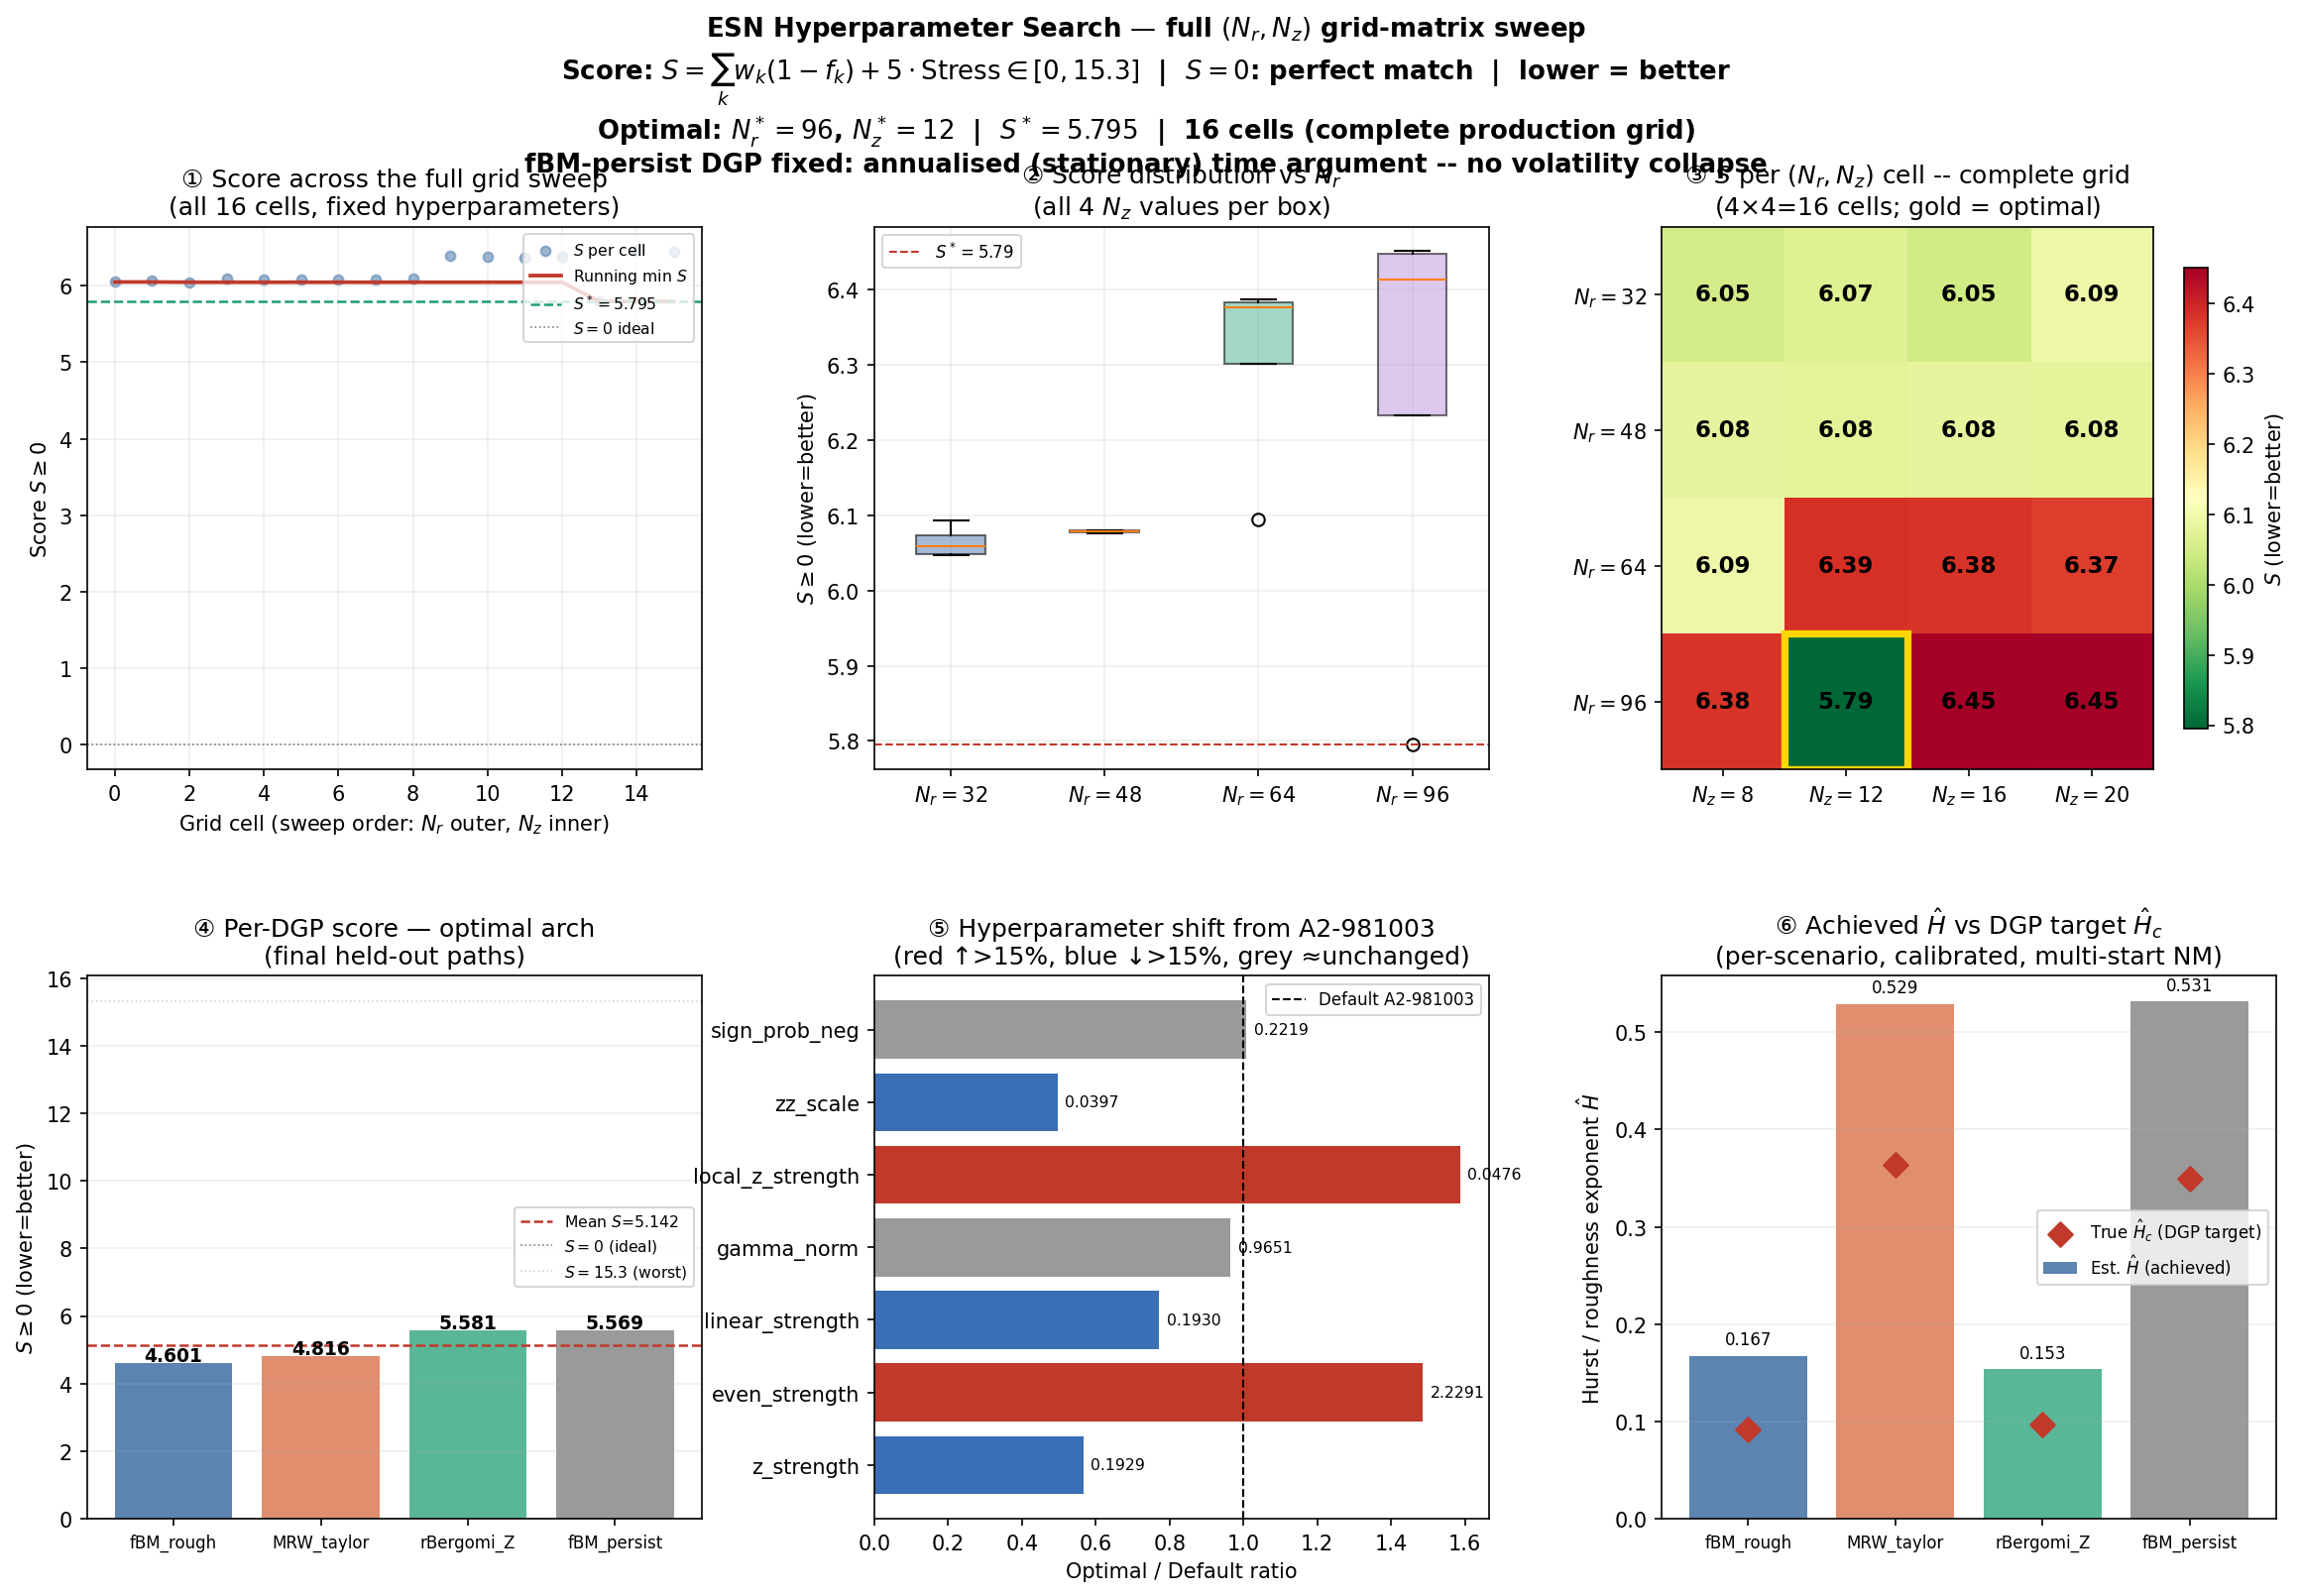
\includegraphics[width=.82\textwidth]{../GridSearch_HyperParameters_Tuning/esn_hyperparam_search_smooth_overview.png}
\end{center}
\vspace{-0.6em}\small\emph{Saved grid-search overview: score and architecture diagnostics are generated by the repository and retained alongside the protocols.}\normalsize

\section{Status, limits, and next validation steps}
The code is a well-developed experiment harness rather than a settled empirical calibration result.  It has explicit DGP sanity checks and fast modes, but no CI, package structure, pinned dependencies, or test suite.  Each protocol copies common machinery, so fixes must be compared before porting.  Results are simulation- and calibration-budget dependent.

Most importantly, the $96\times12$ architecture is not statistically separated from many tested cells at three seeds; single-run Hurst mismatches in the grid report range from 0.056 to 0.182; and the quadratic coefficients $(m_1,m_2)$ are weakly/inconsistently identified across seeds and scenarios.  The sensible next step is a longer, multi-seed, production-budget re-run at a small set of competing reservoir sizes, reporting both $S$ and its 11-term decomposition.  That would test architecture selection, roughness matching, and whether apparent quadratic read-out effects survive calibration noise.

\vspace{.3em}\hrule\vspace{.35em}
\small\textbf{Sources within this repository.} Root \texttt{CLAUDE.md}; \texttt{matteo/web\_claude/CLAUDE.md}; five protocol scripts and their checked-in LaTeX/PDF/PNG outputs.  The latter project-export material supplies research context and document orientation; this report's numerical statements are taken from the protocol reports and JSON outputs.
\end{document}
